\section{Transformer}

\subsection{Output}
\begin{frame}[c]{Output}
    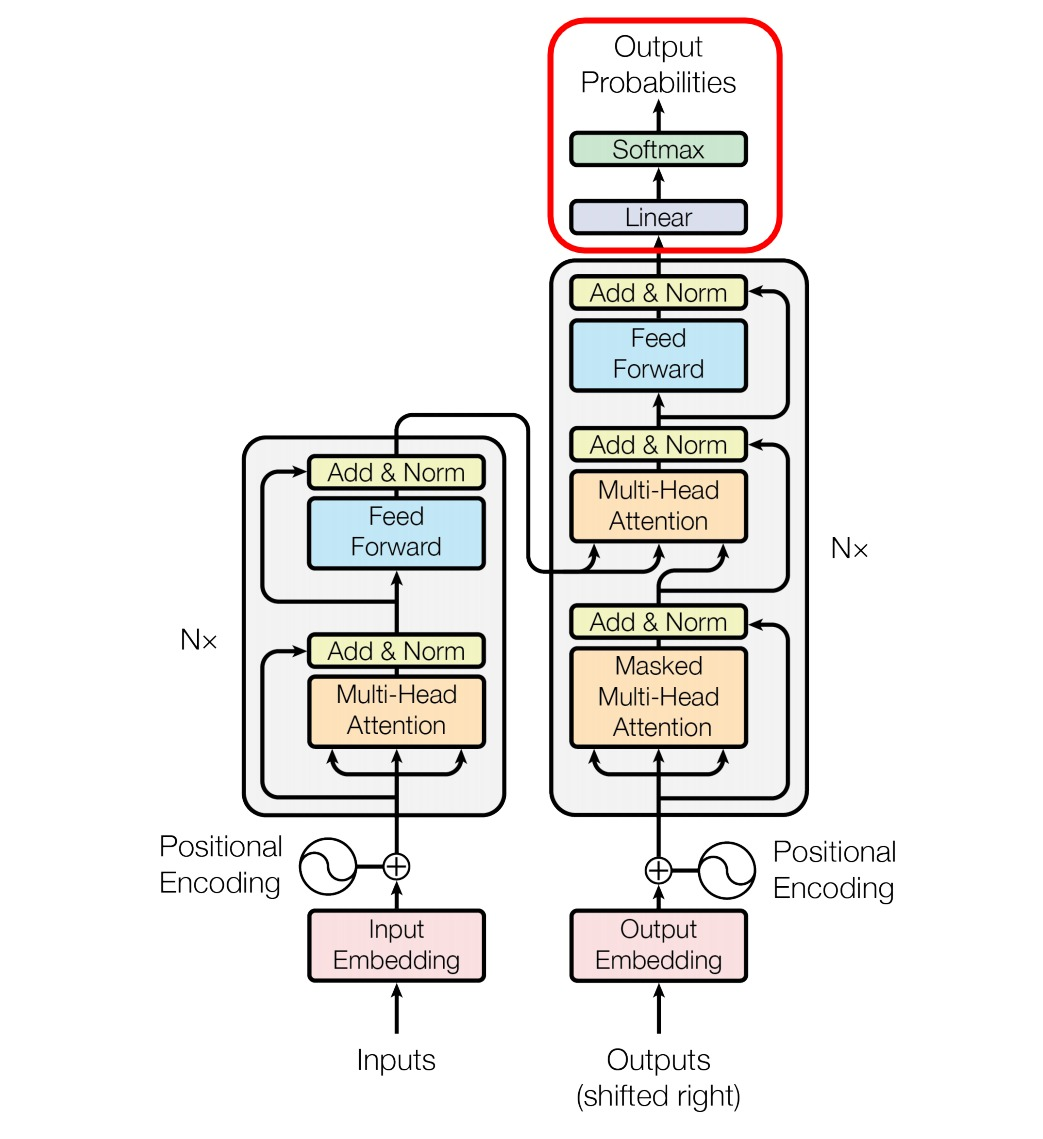
\includegraphics[height=0.9\textheight]{transformer_output}
    \pnote{
    followed by topk selection
    }
\end{frame}

\begin{frame}[c]{Parameters}
    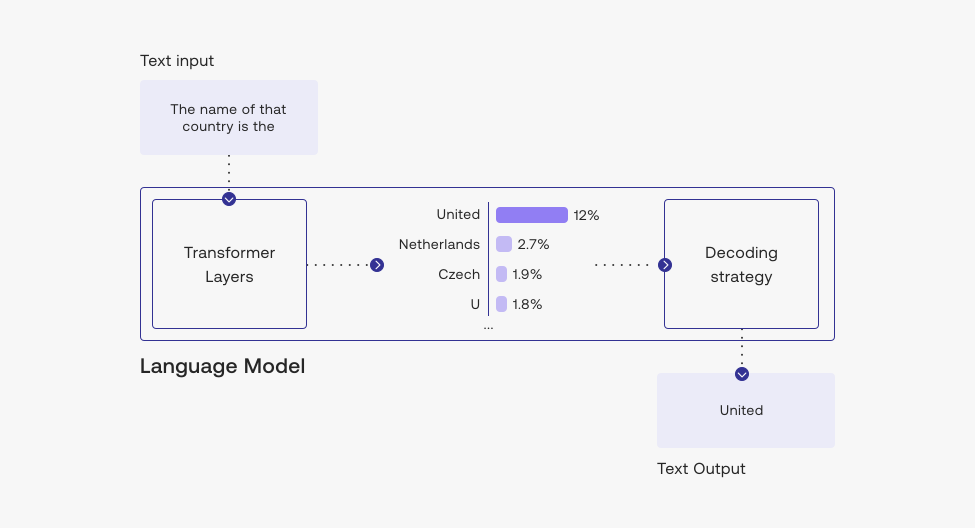
\includegraphics[width=\textwidth]{decoding_strategy} \\
    Image Source: \cite{cohereaidocs_topk_2022}
\end{frame}


\begin{frame}[c]{Temperature, Top-k and Top-p}
    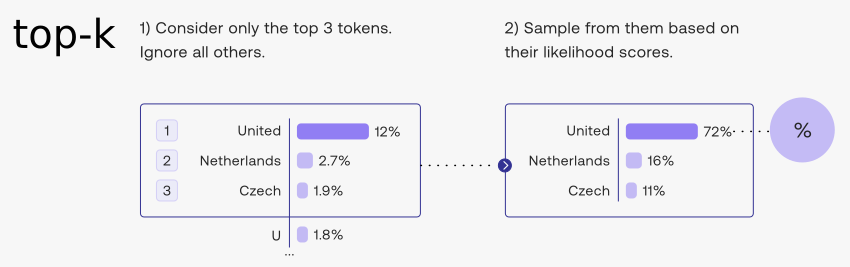
\includegraphics[width=\textwidth]{decoding_topk} \\
    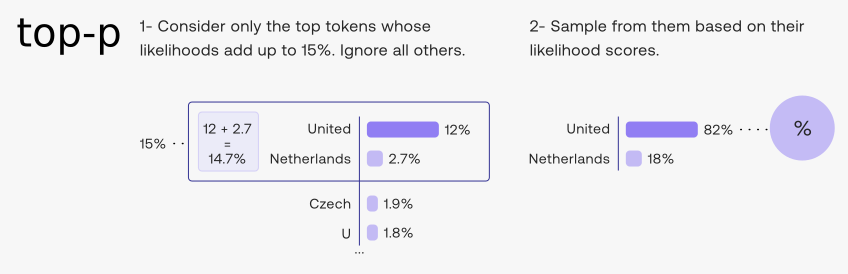
\includegraphics[width=\textwidth]{decoding_topp} \\
    Image Source: \cite{cohereaidocs_topk_2022}
    \pnote{
        Temperature is non-linear rescaling of values, increasing chance of
        lower-likelihood predictions to be chosen.
    }
\end{frame}

\subsection{Dimensions}
\begin{frame}[c]{Dimensions}
    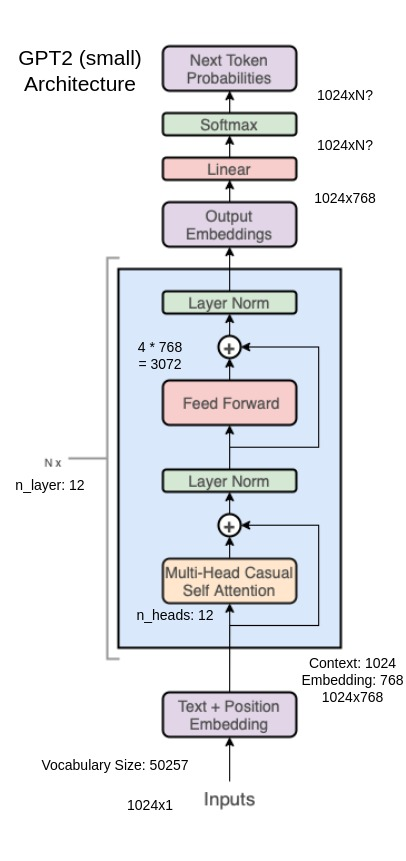
\includegraphics[height=\textheight]{gpt2_decoder_dims}
    Image Adapted from: \cite{gpt_2023}
    \pnote{
        Dimensions represent my current understanding, reality might differ
    }
\end{frame}

\begin{frame}[c]{Dimensions II}
    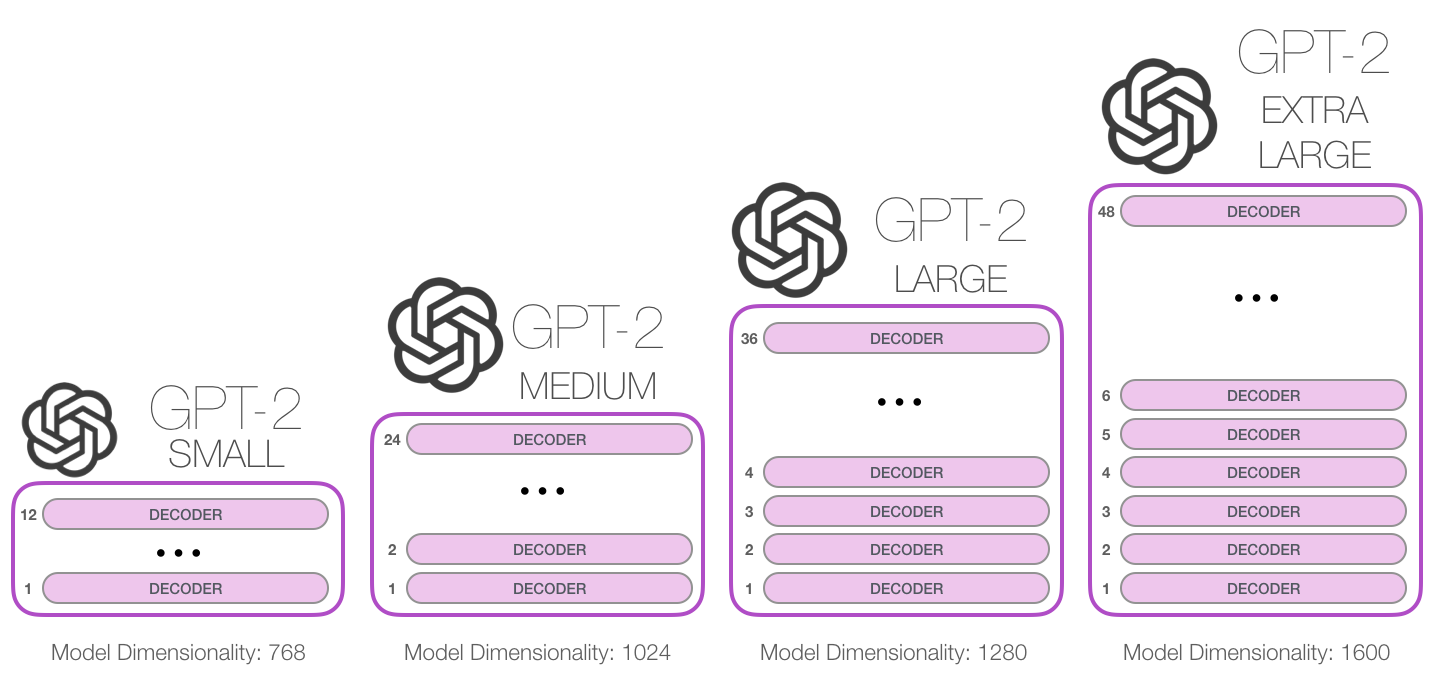
\includegraphics[width=\textwidth]{gpt2-sizes} \\
    Image Source: \cite{alammar_illustrated_2019}
\end{frame}


\subsection{Putting it all Together}
\begin{frame}[c]{Full Architecture}
    \begin{figure}
        \begin{columns}
            \column{0.8\linewidth}
            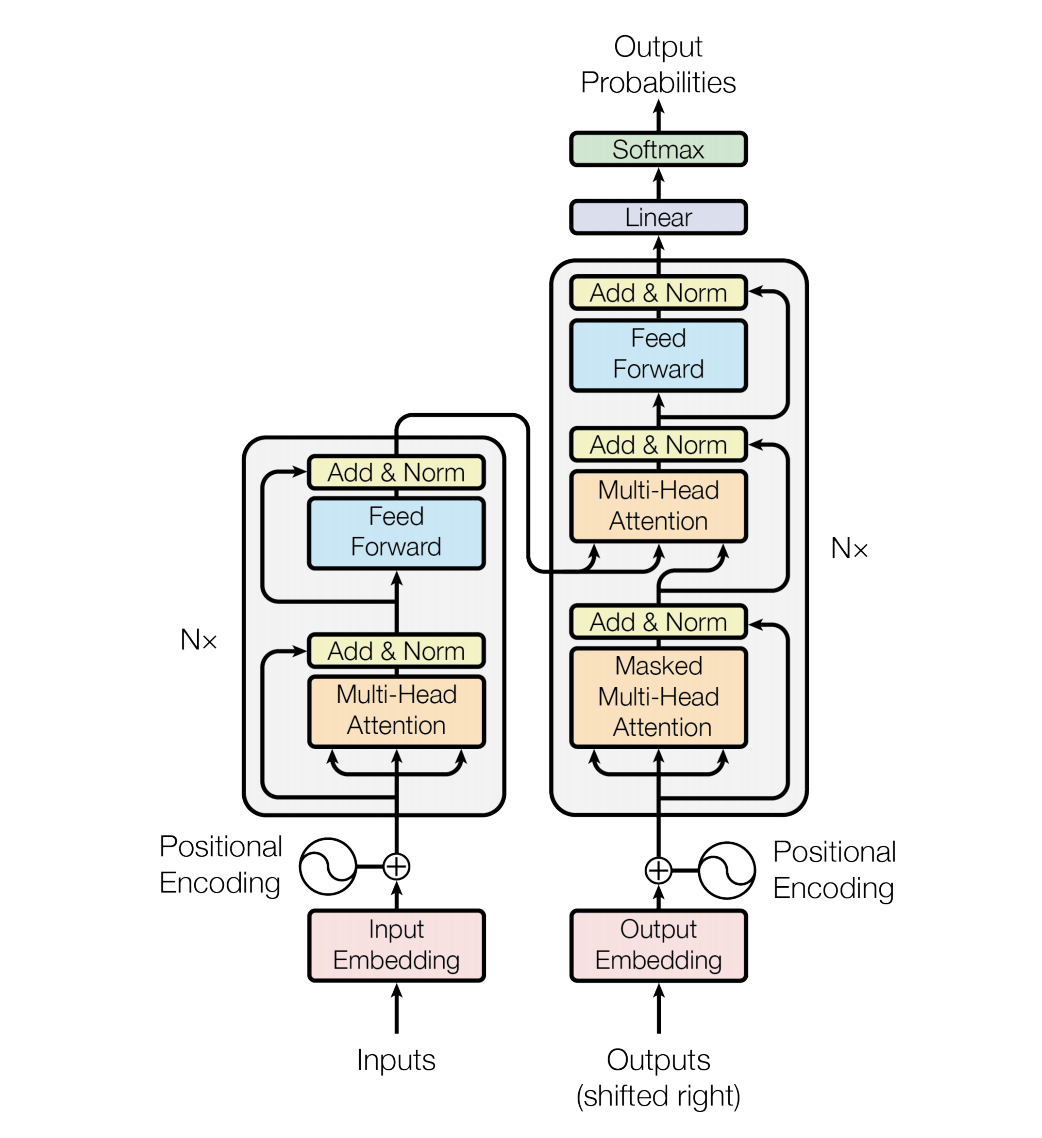
\includegraphics[height=0.9\textheight]{transformer}
            % \column{0.2\linewidth}
            \column{\dimexpr0.15\linewidth+9em}
            \raisebox{3em}{Image Source: \cite{vaswani_attention_2017}}
        \end{columns}
    \end{figure}
\end{frame}

\subsection{Interpretation}
\begin{frame}[c]{One Prevalent Interpretation: Solving ODEs}
    \large
    \begin{aquote}{Lu et al., 2019 \cite{lu_understanding_2019}}
        {\em ... the Transformer can be mathematically interpreted as
        a} numerical Ordinary Differential Equation (ODE) solver for a
        convection-diffusion equation in a multi-particle dynamic
        system.
    \end{aquote}
\end{frame}


\begin{frame}[c]{A Better ODE Solver}
    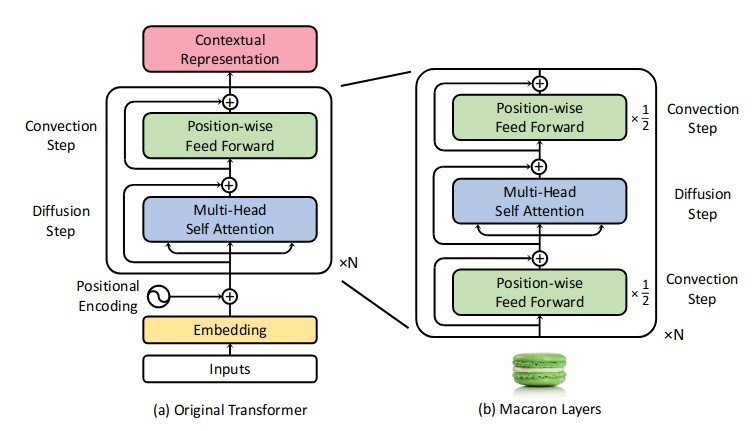
\includegraphics[width=\textwidth]{macaron_layers} \\
    \large
    For solving, use a Strang-Marchuk Splitting scheme instead of Lie-Trotter \\
    \normalsize
    Image Source: \cite{lu_understanding_2019}
    For solving method details, see \cite{geiser_decomposition_2009}
    \pnote{
        they clearly showed that it could be interpreted as physical system
        with particles (tokens) interacting. For that, the solver could be
        improved. \\
        However, while they did improve results, they only did so marginally.
        I assume they didn't use it fully, more experiments necessary.
    }
\end{frame}


\begin{frame}[c]{As High-Order Nonlinearity}
    \large
    \begin{aquote}{Ye et al. 2023, Towards ... \cite{ye_understanding_2023}}
        However, we find only a weak consistency exists between the attention
        weights of features and their importance. We verify the feature map
        multiplication that brings about high-order non-linearity into CNNs is
        crucial for the effectiveness of attention mechanism.
    \end{aquote}
\end{frame}

\subsection{Architecture Improvements}
\begin{frame}[c]{Sparse Transformer: $O(n \sqrt{n})$ instead of $O(n^2)$}
    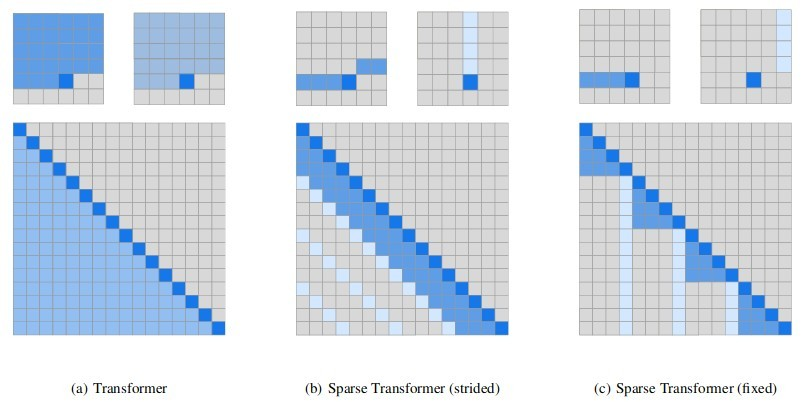
\includegraphics[width=\textwidth]{sparse_transformer} \\
    \normalsize
    Image Source: \cite{child_generating_2019}
    \pnote{
    Even the original GPT didn't use 'full' transformers, but Sparse Transformer \\
    Runtime: O(n sqrt n) instead of O( n * n )
}
\end{frame}


\begin{frame}[c]{FlashAttention}
    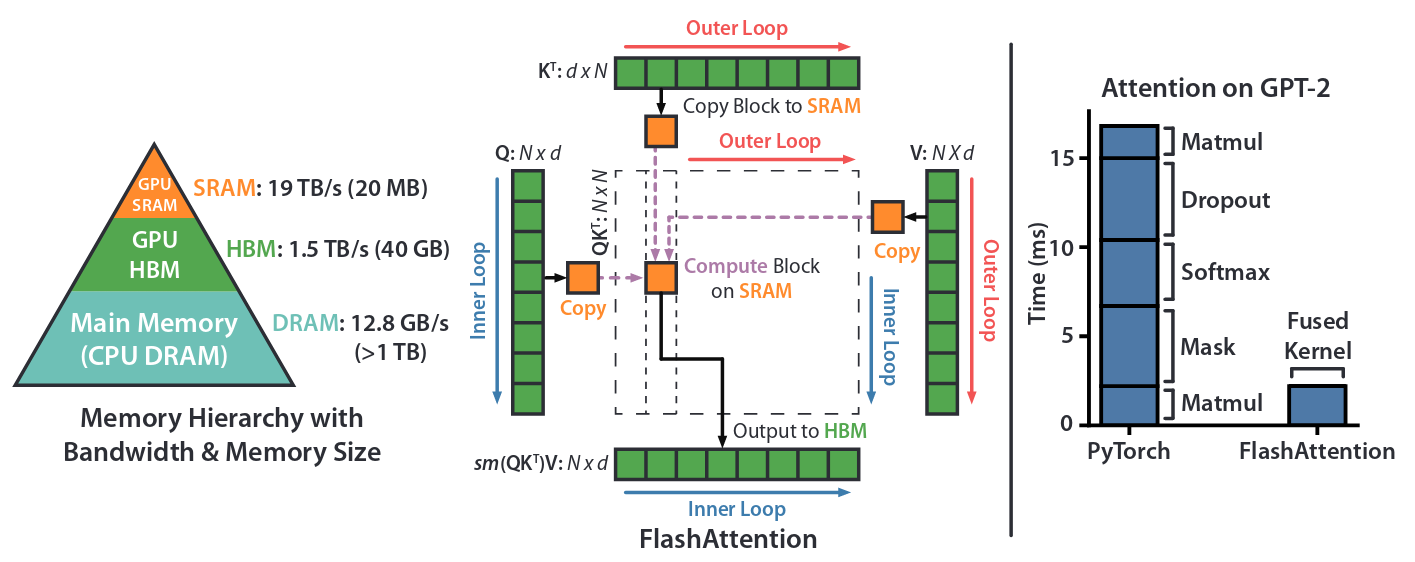
\includegraphics[width=\textwidth]{flashattention_memory} \\
    Image Source: \cite{dao_flashattention_2022}
\end{frame}


\begin{frame}[c]{FlashAttention Benchmarks}
    \large
    \begin{tabular}{c|ccc}
        Attention & Standard & FlashAttention & Ratio \\ \hline
        GFLOPs & 66.6  & 75.2 & 0.89 \\
        HBM R/W & 40.3 & 4.4 & 9.16 \\
        Runtime (ms) & 41.7 & 7.3 & 5.71 \\
    \end{tabular} \newline \newline
    \normalsize
    Table from \cite{dao_flashattention_2022}
\end{frame}

% \begin{frame}[c]{Linear-Time Transformer}
%     FastFormer \cite{wu_fastformer_2021} \\
%     Transformer Quality in Linear Time \cite{hua_transformer_2022} \\
%     \todo{linear time transformer}
% \end{frame}


\begin{frame}[c]{Honorable Mentions}
    \begin{itemize}[<+(1)->]
        \item Transformer-XL \cite{dai_transformerxl_2019}: Attentive Language Models beyond a Fixed-Length Context
        \item Compressive Transformer \cite{rae_compressive_2019}: Long-Range Sequence Modelling by Compressing Past Memories
        \item Memorizing Transformer \cite{wu_memorizing_2022}: kNN-augmented attention layer, can reduce parameter count 5x while keeping perplexity
        \item Adaptive Attention Span \cite{sukhbaatar_adaptive_2019}: varying attention distances
    \end{itemize}
    \pnote{
        Transformer-XL: requires different positional encoding for previous segments \\
        Compressive: 'summarizing' previous segments \\
        Memorizing: on a layer near the top, using xl-based FIFO compression
    }
\end{frame}
